\documentclass[../main.tex]{subfiles}

\begin{document}
\section{Adjustments to the implementation} \label{sec:front-plate-replacement}
Our camera array's casing was originally built using medium-density fibreboard. After some testing, it was clear that the material significantly reduced the potential for a consistent calibration. This is because medium-density fibreboard is simply too bendy to maintain its form. This likely contributed to the poor quality of the original light field renders. Fortunately, we have been able to address this by designing, building, and installing a sturdier aluminium front-plate (see figure~\ref{fig:picam-comparison}). The design specifications for the new front-plate are provided in appendix~\ref{apx:frontplate}. 

\begin{figure}[H]
    \centering
    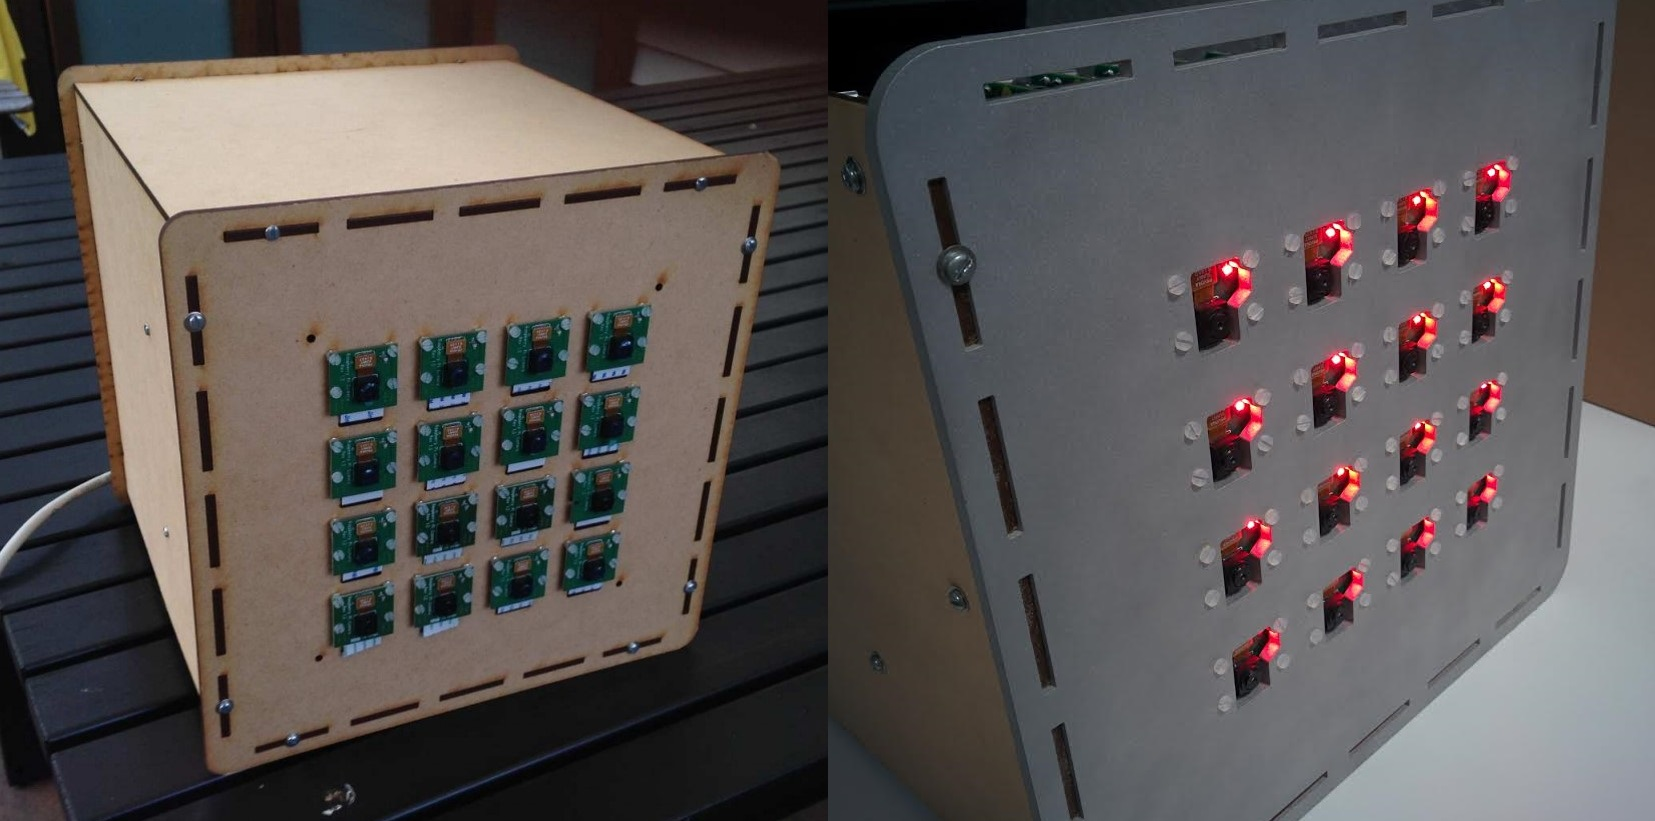
\includegraphics[width=\linewidth]{images/picam-comparison}
    \caption{The original camera array (left) and the camera array with the new aluminium front-plate installed (right).}
    \label{fig:picam-comparison}
\end{figure}

Although the front-plate is now sufficiently sturdy and maintains its form, the cameras themselves still retain some arbitrary rotation (see figure~\ref{fig:rotation-evidence}). This rotation may be due to the nylon nuts and screws used to mount the cameras, which do not fit as tightly as stainless steel materials would. Stainless steel nuts and screws were considered, but were ultimately rejected because they may have damaged the camera boards or caused short-circuits. The cameras themselves may also have some slight variance if they are not built to be absolutely identical. Fortunately, this rotation can be addressed by our novel calibration procedure. 

\end{document}